% +------------------------------------------------------------------------+
% | CGAL Reference Manual:  Subdivision_surfaces_3
% +------------------------------------------------------------------------+
% | Subdivision surfaces on generic Polyhedron.
% | 
% | 1.2.2005  Le-Jeng Andy Shiue
% |
\RCSdef{\subdivisionRev}{$Revision$}
\RCSdefDate{\subdivisionDate}{$Date$}
% +------------------------------------------------------------------------+

\def\CC{Catmull-Clark}
\def\DS{Doo-Sabin}
\def\SQRT3{$\sqrt{3}$}
\def\SUB3{\ccc{Subdivision_surfaces_3}}

% ------------------------------------------------------------------------
\def\FIGDIR{Subdivision_surfaces_3/FIG}
\def\IL{{\itshape left}}
\def\IR{{\itshape right}}
\def\IM{{\itshape middle}}
\def\IT{{\itshape top}}
\def\IB{{\itshape bottom}}
% ------------------------------------------------------------------------

\ccParDims

\chapter{Subdivision Surfaces}
\label{chapterSubdivision}
\ccChapterRelease{\subdivisionRev. \ \subdivisionDate}
\ccChapterAuthor{Le-Jeng Andy Shiue}

\begin{ccTexOnly}
    \setlength{\unitlength}{1mm}
    \begin{picture}(0,0)(0.0,0.0)
      \put (78,25){% textwidth = 156mm
          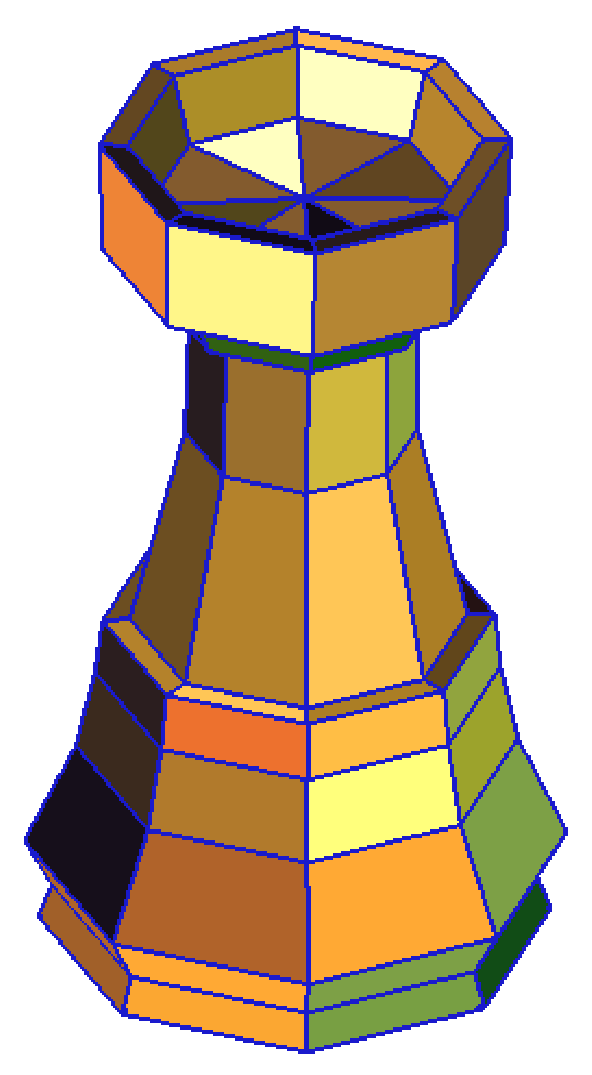
\includegraphics[width=0.1\textwidth]{\FIGDIR/rook_mesh.eps}
          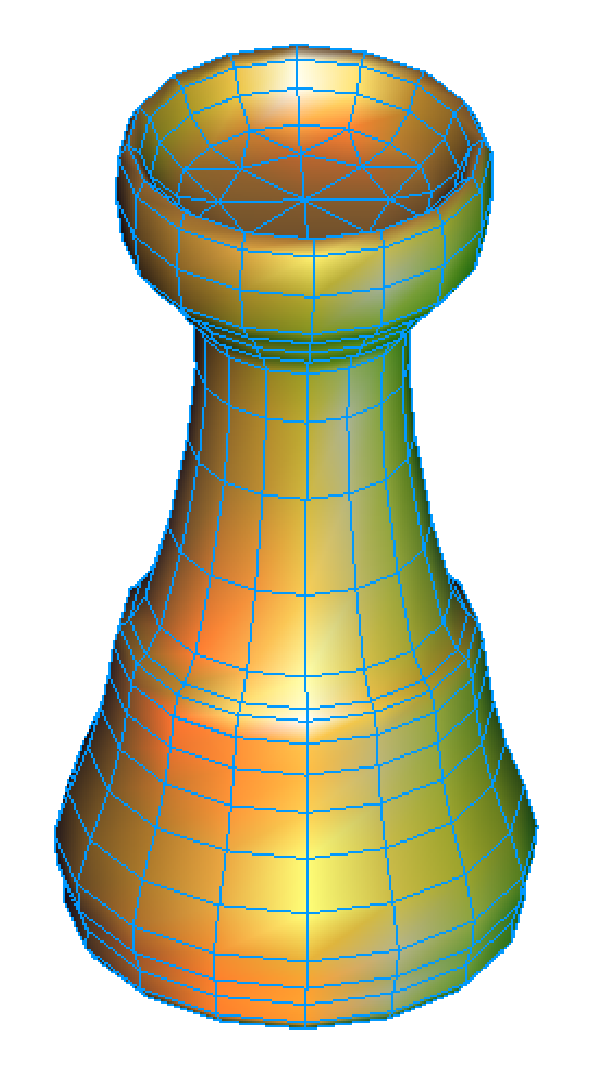
\includegraphics[width=0.1\textwidth]{\FIGDIR/rook_qt1.eps}
          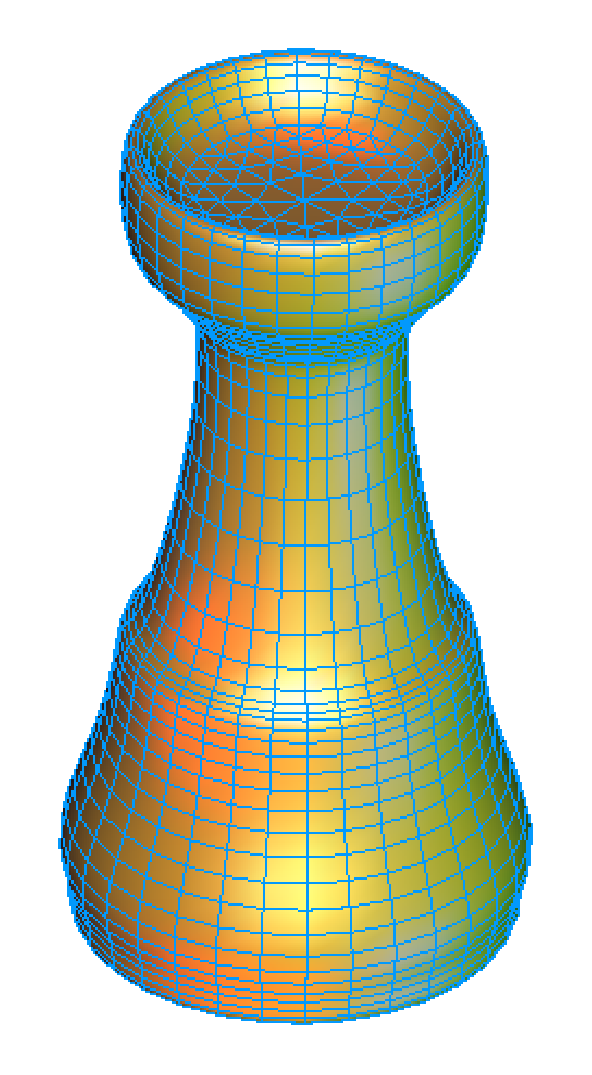
\includegraphics[width=0.1\textwidth]{\FIGDIR/rook_qt2.eps}
          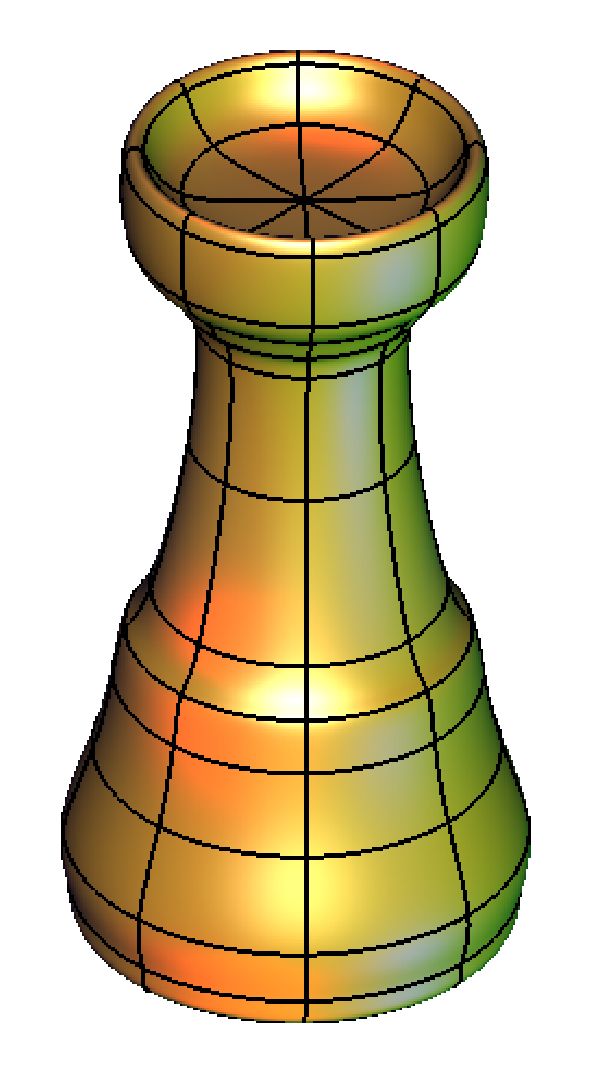
\includegraphics[width=0.1\textwidth]{\FIGDIR/rook_surf1.eps}
          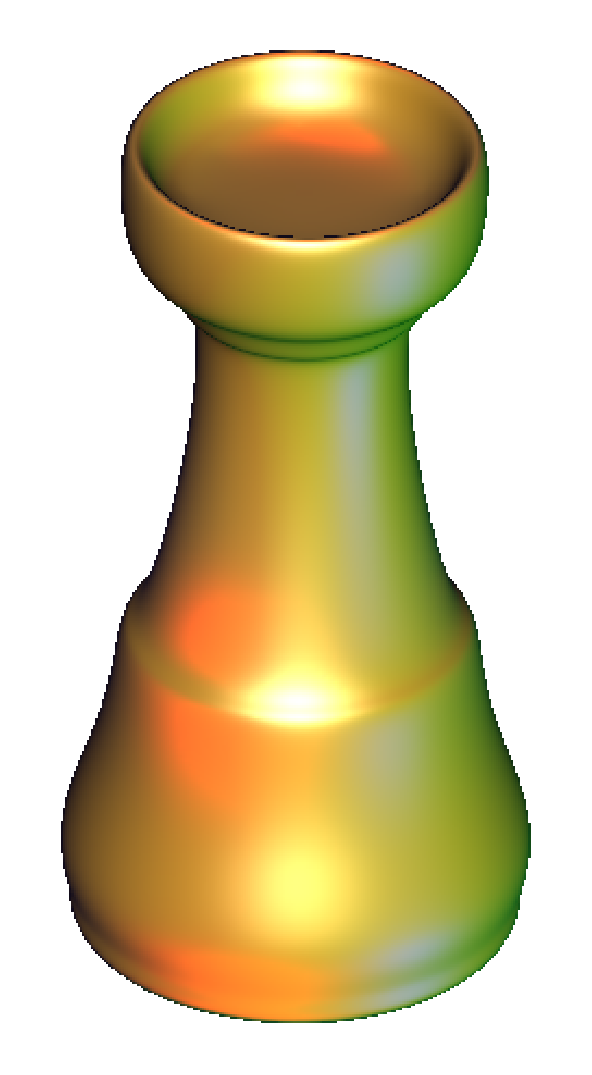
\includegraphics[width=0.1\textwidth]{\FIGDIR/rook_surf2.eps}
      }
    \end{picture}\vspace{-4mm}% compensate for some vspace added by picture
\end{ccTexOnly}

\minitoc

% +------------------------------------------------------------------------+
\section{Introduction} \label{sectionSubIntro}
% +------------------------------------------------------------------------+
Subdivision algorithms (see e.g.\ \cite{Warren-2002-subdivision})
recursively refine coarse meshes and generate ever closer 
approximations to a smooth surface.
%for character animation, surface modeling, or physics simulation. 
Setting aside the specific strategy of geometric averaging
for the new points, subdivision algorithms can be classified 
according to the topological refinement of the underlying mesh.
\SUB3, based on the concept of the 
\ccc{CGAL::Polyhedron_3} (see Chapter~\ref{chapterPolyhedron}),
takes advantage of this separation of topology and geometry, 
and take a cue from the policy-based design \cite{Shiue-2005-SESUB}.

 
%% \begin{ccHtmlOnly}
%%     <CENTER>
%%         <img src="./fig/shark.gif" alt="Hammerhead"><P>
%%     </CENTER>
%% \end{ccHtmlOnly}

%% the combinatorial integrity of them. It is based on the highly
%% flexible design of the halfedge data structure, see the introduction
%% in Chapter~\ref{chapterHalfedgeDS} and~\cite{k-ugpdd-99}. However, the
%% polyhedral surface can be used and understood with


% +------------------------------------------------------------------------+
\section{Subdivision Algorithms}
% +------------------------------------------------------------------------+
Subdivision algorithms define surfaces as the limit
of recursive refinement of a polyhedral mesh. 
%% A mesh is a special graph whose
%% primitives (i.e.~vertices, edges and facets)
%% carry attribute information such as vertex 
%% positions or facet colors. 
The mesh is recursively refined and then smoothed 
by averaging neighbors. The four major refinement 
patterns used in practice are shown in Figure \ref{fig:RefSchemes}.

A graph, called \emph{stencil}, determines the source submesh 
whose nodes contribute to the position of a target node on the
refined mesh. Stencils are defined by the used refinement pattern.
For example, as illustrated in Figure \ref{fig:RefMap},
the PTQ scheme has a vertex-node stencil, which relates the 1-ring 
of a source vertex to a target node, and an edge-node stencil,
which relates the 1-ring of a source edge to a target node; 
while the DQQ scheme has only a corner-node stencil, which 
relates the facet of a corner to a target node.
Stencils with weights are called \emph{geometry stencils}.
The geometry stencils for \CC\ subdivision are
shown in Figure \ref{fig:cc_gstencil}. 
The averaging step positions points of the
refined mesh as a linear combination
of the points on the source submesh and the stencil weights.
The averaging process can typically be factored into 
simpler steps \cite{Oswald-2003-CSS}.
%and this has
%been implemented in the OpenMesh library \cite{Sovakar-2004-APISUB}.
However, while stencil factoring simplifies the implementation,
it is less efficient because it requires repeated visits 
to all nodes.

Since only a fixed number of refinement patterns are practical
but a wide variety of geometry stencils,
\SUB3\ provides refinement patterns (the \emph{refinement hosts})
and hands the definition of geometry stencils
(the \emph{geometry policies}) to the package user.
A subdivision scheme is obtained by parameterizing the refinement
host with geometry policies. 
For example, \CC\ subdivision is instanciated by parameterizing the 
PQQ refinement with the \CC\ geometry stencils.
%\SUB3\ supports 1-ring mesh refinement based on 
%half-edge data structures.
%A subdivision scheme of \ccc{CGAL::Subdivision_surfaces_3} is a 
%refinement host parameterized with a geometry policy. 

%The refinement host realizes the topological refinement and 
%the stencils. The geometry policy consists a set of 
%averaging rules of the geometry stencils.

% +-------------------------------------------------------------+
\subsection{Example: \CC\ Subdivision}
\ccc{CGAL::Subdivision_surfaces_3::PQQ}, the refinement 
host of the PQQ refinement (Figure \ref{fig:RefSchemes}),
realizes the topological refinement and the three stencils
of the PQQ scheme (Figure \ref{fig:RefMap}).

\begin{ccExampleCode}
  // _S is the class implement the geometry policies
  template <template <typename> class _S>
  static void PQQ(Polyhedron& p, _S<Polyhedron> rule, int step)
\end{ccExampleCode}

\SUB3\ provides \ccc{CGAL::CatmullClark_stencil} consisting of the 
geometry policies of the \CC\ subdivision \cite{Catmull-sub-1978}. 
The \CC\ subdivision is then realized by parameterizing 
\ccc{CGAL::Subdivision_surfaces_3::PQQ} with 
\ccc{CGAL::CatmullClark_stencil}.

\begin{ccExampleCode}
  void CatmullClark_subdivision(Polyhedron& p, int step) {
    PQQ(p, CatmullClark_stencil<Polyhedron>(), step);
  }
\end{ccExampleCode}

\ccc{Polyhedron} is the template parameter of the concept of
\ccc{CGAL::Polyhedron_3}, and \ccc{step} specifies the
depth of the subdivision.


%Catmull-Clark, Loop, Doo-Sabin and $\sqrt{3}$ subdivisions are supported
%in \ccc{CGAL::Subdivision_surfaces_3} as convenient functions.

% +-------------------------------------------------------------+
\section{Refinement Host}
\SUB3\ current provides four refinement hosts of primal 
quadrilateral quadrisection (PQQ), primal triangle 
quadrisection (PTQ), dual quadrilateral 
quadrisection (DQQ) and \SQRT3 triangulation, which 
are used by \CC, Loop, \DS\ and \SQRT3\ subdivision, 
respectively. The refined mesh is shown below 
the initial mesh.

\begin{ccTexOnly}
  \begin{center}
    \parbox{0.6\textwidth}{%
      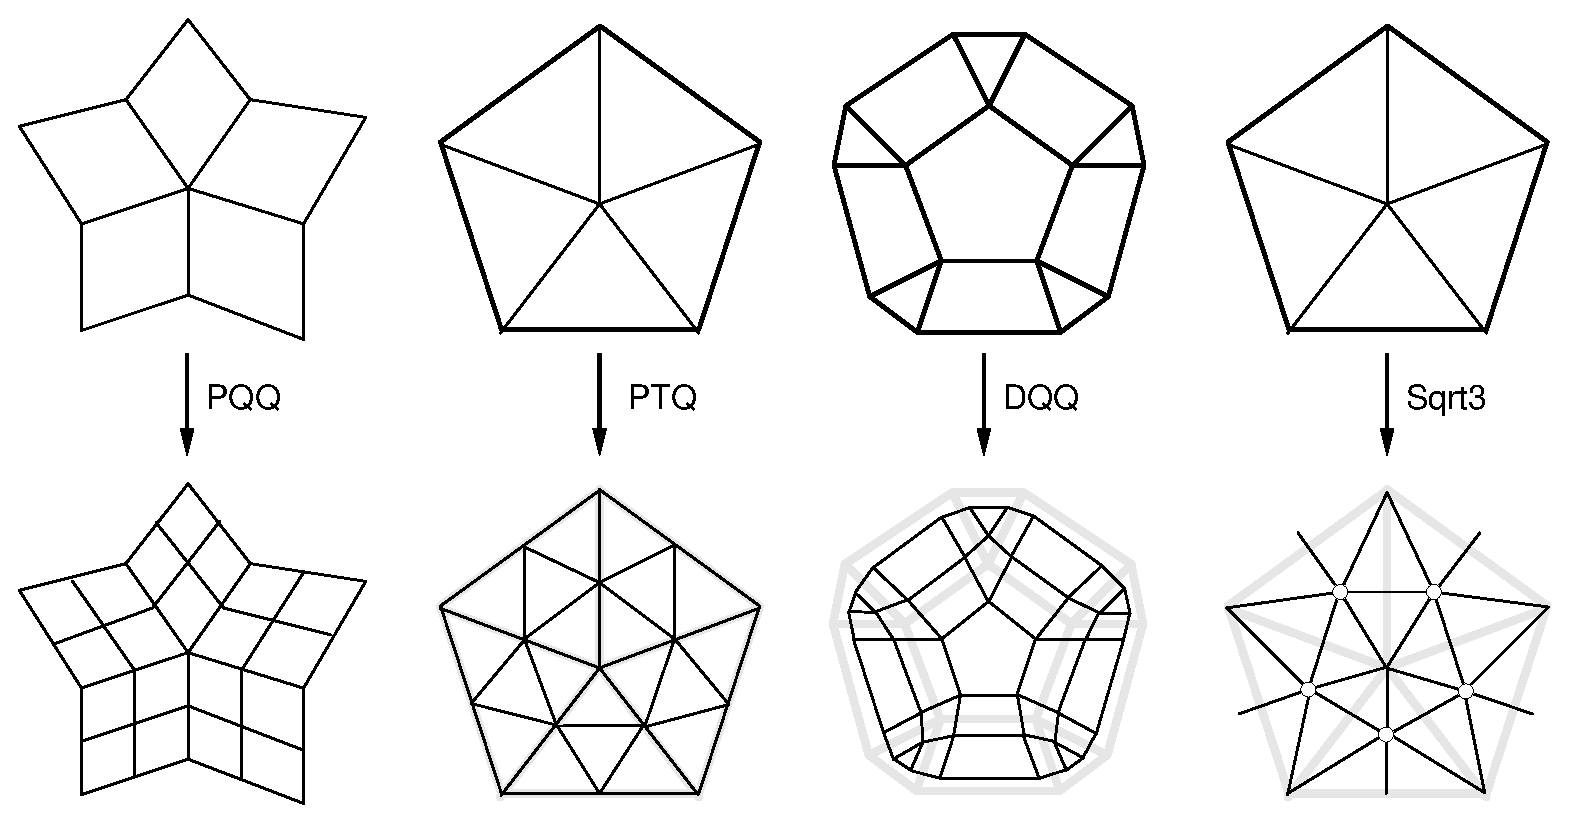
\includegraphics[width=0.6\textwidth]{\FIGDIR/RefSchemes.eps}%
    }
  \end{center}
\end{ccTexOnly}

\begin{ccHtmlOnly}
  <CENTER>
  <A HREF="./FIG/RefSchemes.gif">
     <img src="./FIG/RefSchemes.gif" alt="Refinement Hosts"></A><P>
  </CENTER>
\end{ccHtmlOnly}

%% Stencils are maintained using the iteration concept
%% to avoid the need for vertex tags to distinguish
%% the stencil types.
%% For example, on a PQQ refined mesh, the vertex iterator 
%% visits the 
%% vertex-nodes, edge-nodes and then facet-nodes. The visit
%% order is implicitly used to determine the stencil of
%% the visited node.

Each refinement host is realized as a static function of
a refining polyhedron and a geometry policy. Refinement hosts
are responsible to maintain the stencils by the ordering of 
the new nodes. Interested users should refer to \cite{Shiue-2005-MREO} 
for details of the ordering algorithm.

\begin{ccExampleCode}
template <class Polyhedron>
class Subdivision_surfaces_3 {
  // _S is the class implement the geometry policies
  template <template <typename> class _S>
  static void PQQ(Polyhedron& p, _S<Polyhedron> rule, int step);

  template <template <typename> class _S>
  static void PTQ(Polyhedron& p, _S<Polyhedron> rule, int step);

  template <template <typename> class _S>
  static void DQQ(Polyhedron& p, _S<Polyhedron> rule, int step);

  template <template <typename> class _S>
  static void Sqrt3(Polyhedron& p, _S<Polyhedron> rule, int step);
}
\end{ccExampleCode}

% +-------------------------------------------------------------+
\section{Geometry Policy}
A class of geometry policies defines a set of functions 
of the geometry averaging rules to assign the new node 
according to the source stencil..
%The policy interface is defined with the refinement host. 
Each function of the geometry rules receives a primitive handle 
of the source mesh, and the target node as the reference of 
the \ccc{Point}. Developers of the geometry policy collect the submesh
of the primitive handle, and caculate the new node by averaging
the weighted submesh. 

A PQQ reinement host requires three geometry policies for closed 
surfaces (i.e.~surfaces without boundaries):  a vertex-node stencil 
of a source vertex, an edge-node stencil of a source edge, and a 
facet-node stencil of a source facet.

\begin{ccTexOnly}
  \begin{center}
    \parbox{0.5\textwidth}{%
      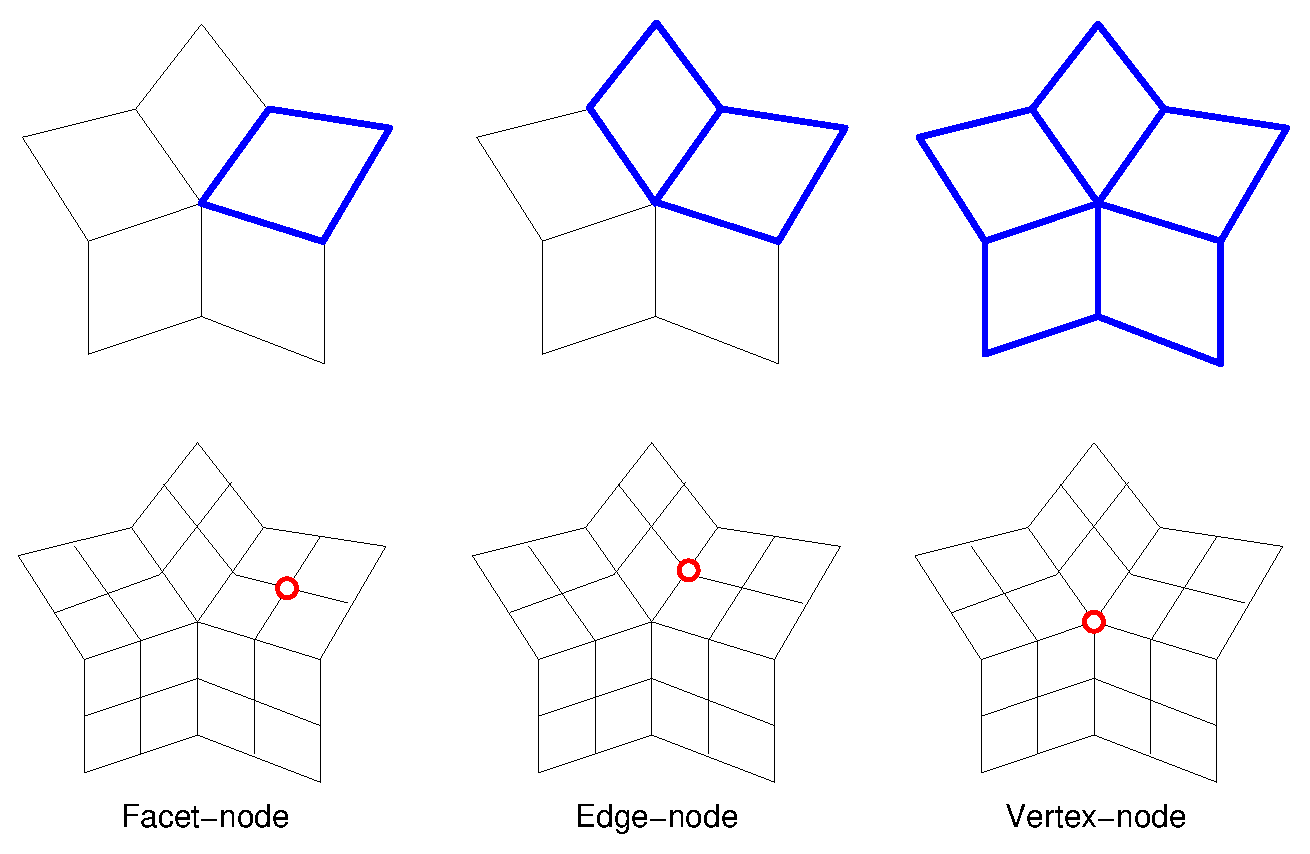
\includegraphics[width=0.5\textwidth]{\FIGDIR/PQQStencil.eps}%
    }
  \end{center}
\end{ccTexOnly}

\begin{ccHtmlOnly}
  <CENTER>
  <A HREF="./FIG/PQQStencil.gif">
     <img src="./FIG/PQQStencil.gif" alt="Stecils of PQQ scheme "></A><P>
  </CENTER>
\end{ccHtmlOnly}

Following shows the realization of the \CC\ rules as geometry policy class.
To support meshes with boundary, an additional policy for 
border vertices is required.

\begin{ccExampleCode}
template <class _Poly>
class CatmullClark_stencil {
   void edge_node(Halfedge_handle edge, Point& pt) {
    Point p1 = edge->vertex()->point();
    Point p2 = edge->opposite()->vertex()->point();
    Point f1, f2;
    facet_node(edge->facet(), f1);
    facet_node(edge->opposite()->facet(), f2);
    pt = Point((p1[0]+p2[0]+f1[0]+f2[0])/4,
               (p1[1]+p2[1]+f1[1]+f2[1])/4,
               (p1[2]+p2[2]+f1[2]+f2[2])/4 );
  }
 
  void vertex_node(Vertex_handle vertex, Point& pt) {
    Halfedge_around_vertex_circulator vcir = vertex->vertex_begin();
    int n = circulator_size(vcir);    

    float Q[] = {0.0, 0.0, 0.0}, R[] = {0.0, 0.0, 0.0};
    Point& S = vertex->point();
    
    Point q;
    for (int i = 0; i < n; i++, ++vcir) {
      Point& p2 = vcir->opposite()->vertex()->point();
      R[0] += (S[0]+p2[0])/2;
      R[1] += (S[1]+p2[1])/2;
      R[2] += (S[2]+p2[2])/2;
      facet_node(vcir->facet(), q);
      Q[0] += q[0];      
      Q[1] += q[1];      
      Q[2] += q[2];
    }
    R[0] /= n;    R[1] /= n;    R[2] /= n;
    Q[0] /= n;    Q[1] /= n;    Q[2] /= n;
      
    pt = Point((Q[0] + 2*R[0] + S[0]*(n-3))/n,
               (Q[1] + 2*R[1] + S[1]*(n-3))/n,
               (Q[2] + 2*R[2] + S[2]*(n-3))/n );
  }

  void border_node(Halfedge_handle edge, Point& ept, Point& vpt) {
    Point& ep1 = edge->vertex()->point();
    Point& ep2 = edge->opposite()->vertex()->point();
    ept = Point((ep1[0]+ep2[0])/2, (ep1[1]+ep2[1])/2, (ep1[2]+ep2[2])/2);

    Halfedge_around_vertex_circulator vcir = edge->vertex_begin();
    Point& vp1  = vcir->opposite()->vertex()->point();
    Point& vp0  = vcir->vertex()->point();
    Point& vp_1 = (--vcir)->opposite()->vertex()->point();
    vpt = Point((vp_1[0] + 6*vp0[0] + vp1[0])/8,
                (vp_1[1] + 6*vp0[1] + vp1[1])/8,
                (vp_1[2] + 6*vp0[2] + vp1[2])/8 );
  }
}
\end{ccExampleCode}

%% \begin{ccExampleCode}
%% PQQ<_M,CCstencil>(Mesh,CCstencil<_M>())
%% \end{ccExampleCode}
%% (or, more simply \\
%% \begin{ccExampleCode}
%% PQQ(Mesh,CCstencil<_M>())}
%% \end{ccExampleCode}
%% since the compiler can derive the template
%% arguments from the function parameters),
%% instantiates \CC\ subdivision.    
%% \ccc{_M}, the model of the mesh concept,
%% represents the mesh type (\ccc{Mesh}),
%% and \ccc{CCstencil} is a class template 
%% realizing geometry policies of \CC\ subdivision.

The geometry stencils of \CC\ subdivision (border stencils are 
not included) are shown below. 

\begin{ccTexOnly}
  \begin{center}
    \parbox{0.4\textwidth}{%
      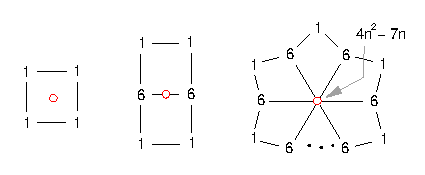
\includegraphics[width=0.4\textwidth]{\FIGDIR/cc_mask.eps}%
    }
  \end{center}
\end{ccTexOnly}

\begin{ccHtmlOnly}
  <CENTER>
  <A HREF="./FIG/cc_mask.gif">
     <img src="./FIG/cc_mask.gif" alt="\CC\ geometry stencil"></A><P>
  </CENTER>
\end{ccHtmlOnly}


% +------------------------------------------------------------------------+
\section{Bult-in subdivisions}
% +------------------------------------------------------------------------+
\CC , Loop, \DS\ and \SQRT3\ subdivisions are provided in \SUB3. Each of these 
subdivision schemes is realized with the corresponding geometry policies.
\begin{ccExampleCode}
  static void CatmullClark_subdivision(Polyhedron& p, int step) {
    PQQ(p, CatmullClark_stencil<Polyhedron>(), step);
  }
  static void Loop_subdivision(Polyhedron& p, int step) {
    PTQ(p, Loop_stencil<Polyhedron>() , step);
  }
  static void DooSabin_subdivision(Polyhedron& p, int step) {
    DQQ(p, DooSabin_stencil<Polyhedron>(), step);
  }
  static void Sqrt3_subdivision(Polyhedron& p, int step) {
    Sqrt3(p, Sqrt3_stencil<Polyhedron>(), step);
  }
\end{ccExampleCode}

Following shows an example of \DS\ subdivision on a polyhedral mesh.
\ccIncludeExampleCode{Subdivision_surfaces_3/DooSabin_subdivision.C}

% +------------------------------------------------------------------------+
\section{Customize subdivision surfaces}
% +------------------------------------------------------------------------+
To develop a customized subdivision scheme, users first choose a 
refinement host for the topological refinement, and then implement 
the geometry policies accordingly. 
The following exmple develops a subdivsion scheme
generating improved Loop subdivision surfaces based on the PTQ refinement 
(i.e~\ccc{Subdivision_surfaces_3<Polyhedron>::PTQ}). The policy class of
the user-defined geometry rules is deveoped as a subclass 
of \ccc{PTQ_stencil}), which defines the interface of stencils
of the PTQ refinement. A policy function for subdivision 
surfaces is semantically required to assigned the smoothed point 
based on the source mesh. 

\ccIncludeExampleCode{Subdivision_surfaces_3/Customized_subdivision.C}
